\newgeometry{left=4.5cm, right=4.5cm,bottom=4cm, top=4cm}
\chapter{The ATLAS Detector at the LHC}\label{chap:detector}
 \vspace{0.5cm}

The Large Hadron Collider (LHC) located at the European Organisation for Nuclear Research (CERN) in Geneva, Switzerland,
is  the largest particle collider facility in the world, colliding protons and heavy ions at the so far largest centre-of-mass
energies. The ATLAS experiment is one of the experiments at the LHC designed  to search for  a wide range of new 
physics phenomena and to perform  precision measurements of Standard Model processes.
Proton-proton collision data recorded by the ATLAS detector in 2012  has been used for 
the search for the neutral MSSM Higgs bosons presented in this thesis.

The chapter is organised as follows: the design and performance of the LHC  are summarised in 
Section~\ref{sec:lhc}, based on~\cite{LHC},  while  the  ATLAS detector  is 
described in Section~\ref{sec:atlas}, based on~\cite{ATLASDetector}.


\restoregeometry
\clearpage



\section{The Large Hadron Collider}\label{sec:lhc}
The LHC is a hadron synchrotron  collider with superconducting magnets. 
It is  installed in the tunnel of the former Large Electron-Positron collider (LEP)
with a circumference of about $27$~km.
LHC is designed to collide proton beams at a  centre-of-mass energy of 14 TeV and an unprecedented peak luminosity of 
$10^{34} ~ \text{cm}^{-2} \text{s}^{-1}$. It can also collide heavy ion (lead) beams carrying  an energy of 2.8 TeV per nucleon at
a peak luminosity of $10^{27} ~ \text{cm}^{-2} \text{s}^{-1}$. 

Figure~\ref{fig:LHC} shows the layout of the CERN accelerator complex. The  protons undergo several acceleration steps before 
injection into the LHC machine.
A linear  accelerator ($Linac\,2$) brings the protons to an energy of 50~MeV at  which
they are injected into the \emph{Booster} where they are  further  accelerated
to 1.4~GeV. The proton energy is successively increased to 25~GeV and to 450~GeV in the \emph{Proton Synchrotron} (PS)
and the \emph{Super Proton Synchrotron} (SPS), respectively. Finally the protons are  injected in two
opposite directions into the LHC ring where they reach their final energy.

The proton beams are  housed in two separate vacuum pipes and consist of up to 2835 proton bunches, each
of them containing about $10^{11}$ protons. 
Radiofrequency cavities are employed  to accelerate the protons
while superconducting magnets bend and focus the beams.
The nominal bunch spacing allows for bunch crossings  every 25~ns which represents a challenge for the detector read-out electronics.

First proton-proton collisions took place at the LHC in 2009 at a centre-of-mass  energy of 900~GeV
followed by collision at 7~TeV in 2010. The LHC successfully delivered
 data with increasing instantaneous luminosity during the years 2011 and 2012. 
The  centre-of-mass  energy was increased to 8~TeV in 2012.
Peak luminosities of about $4\times10^{33} ~ \text{cm}^{-2}\text{s}^{-2}$ 
and $8\times10^{33} ~ \text{cm}^{-2}\text{s}^{-2}$  have been reached 
in years 2011 and 2012, respectively.
The physics program of the LHC is carried out  by four major experiments,  ATLAS~\cite{ATLASDetector}, CMS~\cite{cms},
LHCb~\cite{lhcb} and ALICE~\cite{alice}. 
The ATLAS experiment recorded proton-proton collision data corresponding to an integrated luminosity of 4.57~$\text{fb}^{-1}$ 
during 2011 and additional  20.3~$\text{fb}^{-1}$ during 2012.
The data recorded during  these two years  led to one of the major milestones
 in particle physics, the discovery of  a Higgs boson with a mass of about $125$~GeV.





\begin{figure}[tp]
     \begin{center}

            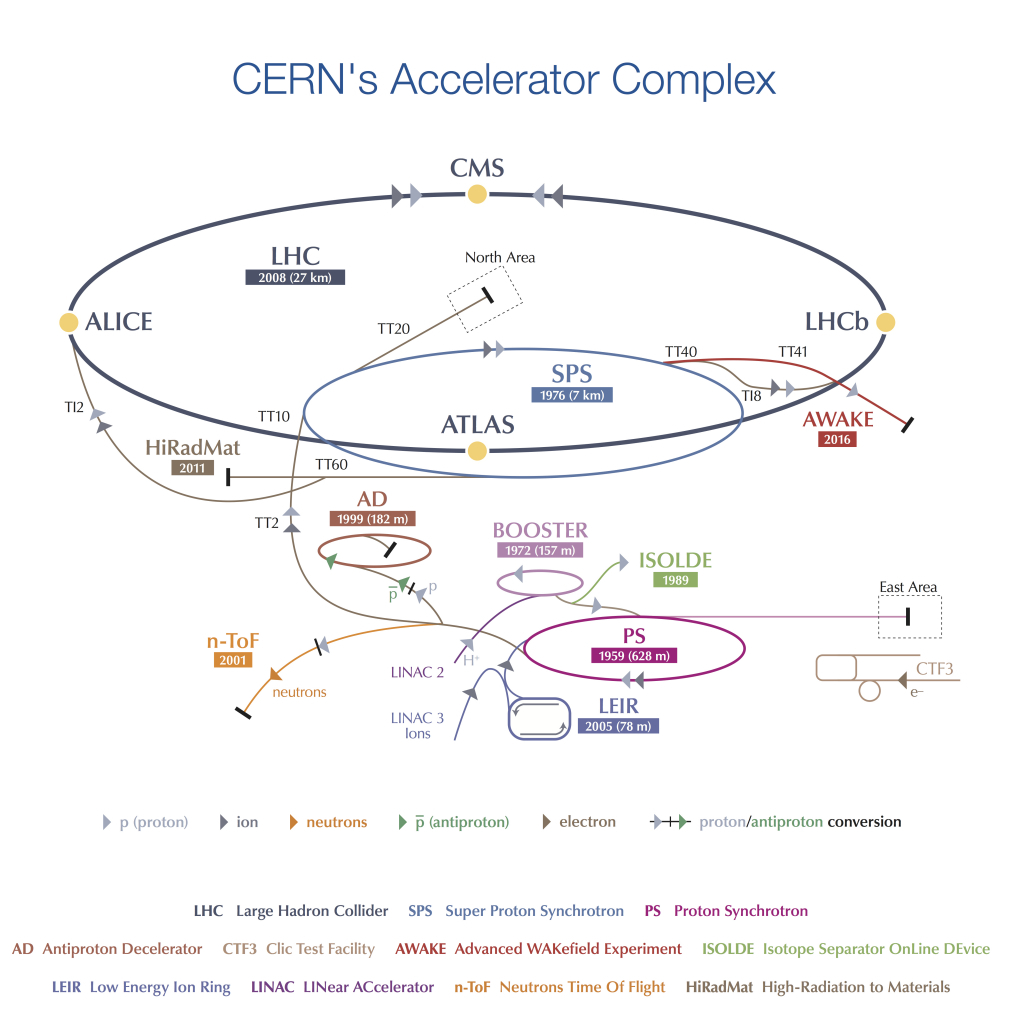
\includegraphics[width=\textwidth]{figure/LHC2.jpg}

    \end{center}
    \caption{Illustration of the CERN accelerator complex~\cite{lhcImage}. The acceleration of the 
	protons starts in Linac2 followed by the Booster. The Proton Synchrotron (PS) and the Super Proton 
	Synchrotron (SPS) further accelerate the protons until their final injection into the LHC, 
	where they acquire their final collision energy.}


   \label{fig:LHC}
\end{figure}


\section{The ATLAS Detector}\label{sec:atlas}
The ATLAS detector is a multi-purpose detector aiming to explore a wide range of physics 
phenomena at the Teraelectronvolt energy scale.
The physics goals impose strong requirements on particle reconstruction efficiency and accuracy.
A schematic view of the ATLAS detector is shown in Figure~\ref{fig:atlas}$\,.$ 
With a length of $44\,$m and a height of $25\,$m it is the largest detector at the LHC, 
it is installed at one of the LHC interaction points about
100 below ground. ATLAS consists of four sub-detectors which are installed  cylindrically around the
beam pipe in the central barrel part and 
in disks in the endcap parts which are symmetrically in the forward and backward direction with respect to the proton beams.
The innermost sub-detector is the inner detector (ID), followed by the electromagnetic calorimeter, the hadronic calorimeter and finally
the muon spectrometer (MS) in the outermost layer. Each of these sub-detectors is briefly described below
 based on  reference~\cite{ATLASDetector}.


\begin{figure}[tp]
     \begin{center}

            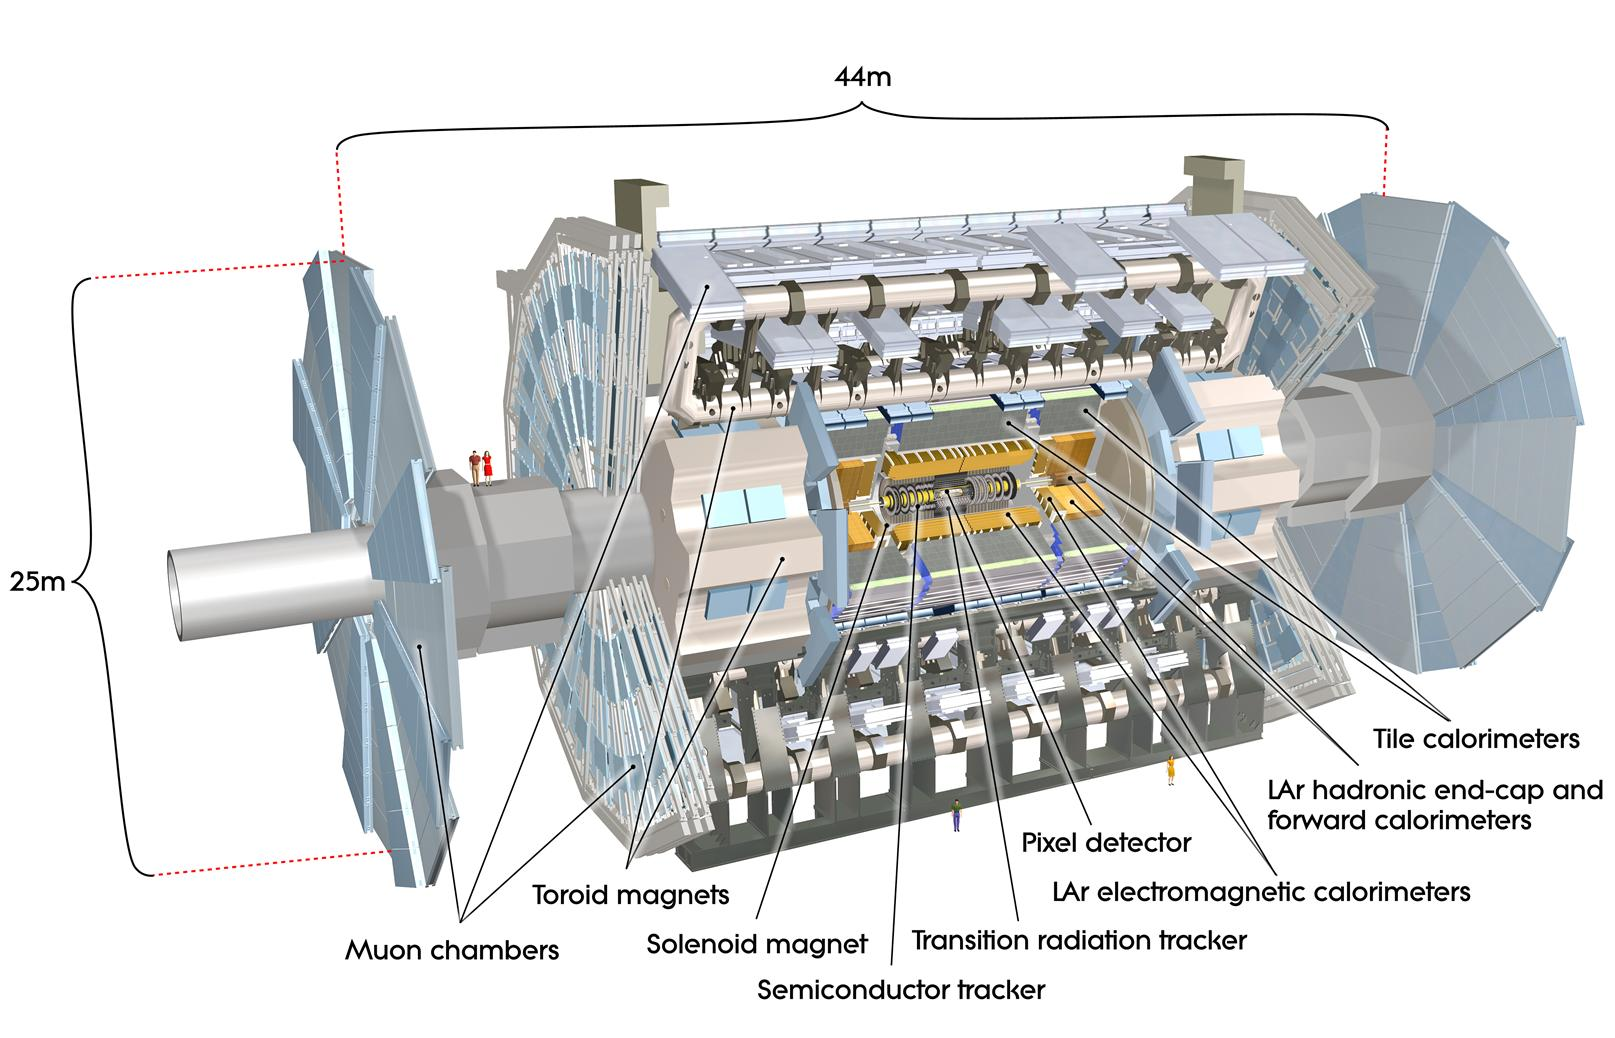
\includegraphics[width=\textwidth]{figure/ATLAS.jpeg}

    \end{center}
    \caption{Cut-away view of the ATLAS detector with its sub-detectors~\cite{ATLASDetector}.}



   \label{fig:atlas}
\end{figure}


\subsection{The ATLAS coordinate system}
\begin{figure}[!tp]
     \begin{center}

            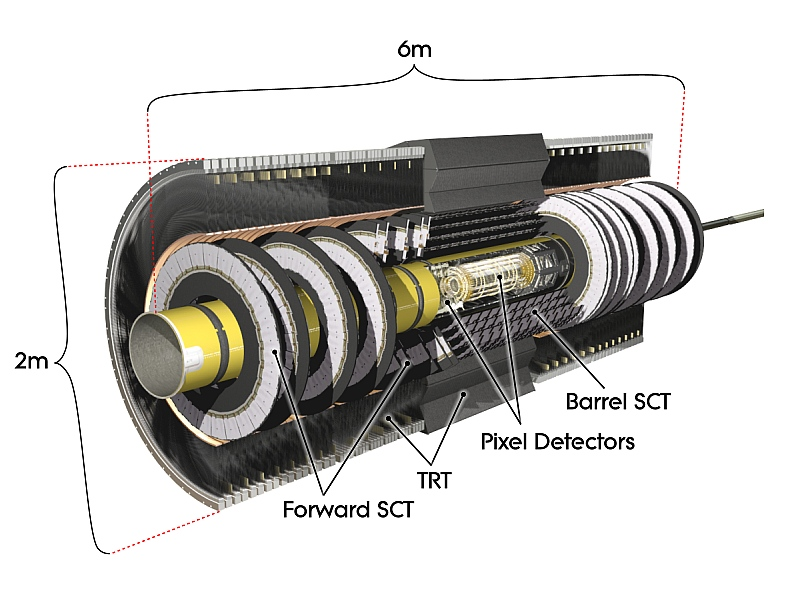
\includegraphics[width=0.8\textwidth]{figure/Inner_detector.jpg}

    \end{center}
    \caption{Cut-away view of the ATLAS inner detector~\cite{ATLASDetector}.}

   \label{fig:atlasID}
\end{figure}

The right-handed ATLAS coordinate system has its origin at the interaction point. The $z-$axis is pointing along the
beam direction, the $y-$axis  upwards and the $x-$axis towards the centre of the LHC ring. 
The azimuthal angle $\phi$ is defined in the transverse plane orthogonal
to the beam axis starting from the positive side of the $x-$axis. The polar angle $\theta$ is  defined with respect to the $z-$axis.

A commonly used kinematical variable at  collider experiments  is the rapidity
\begin{equation}
y ~ = ~ 1/2 \cdot \ln \left( \frac{E + p_{z}}{E - p_z} \right) \,, 
\end{equation}
where $E$ and $ p_z$ are the particle energy and the momentum component in  $z$-direction, respectively.
The difference in  rapidity of two particles is independent of Lorentz boosts along the beam axis. 
In the limit where the particle velocity approaches  the speed of light and
 for massless particles the rapidity can be approximated by the pseudo rapidity
\begin{equation}
\eta ~ = ~ 1/2 \cdot \ln \left( \frac{\theta}{2} \right)\,. 
\end{equation}
The ATLAS detector is divided into the \emph{barrel} region with  cylindrical geometry
extending up to $|\eta| \apprle 1.5$ (depending on the particular  sub-detector) 
and the \emph{endcap} regions with a disk structure at larger~$\eta$ values. The angular separation between 
two particles is commonly measured by
 $\Delta R ~=~\sqrt{\Delta \eta^2 + \Delta \phi^2}\,$, where $\Delta\eta$ and $\Delta\phi$ are the difference in pseudo rapidity
and azimuthal angle between the particles, respectively.
%Given the symmetry 
%of the ATLAS detector, it is divided in two regions, barrel and endcap.

\subsection{The Inner Detector}


In the inner detector  curved trajectories of charged particles are reconstructed in a 2\,T solenoidal magnetic field
providing measurements of the particle momenta and of  the position of the interaction vertices. 
The layout of the inner detector is illustrated in Figure~\ref{fig:atlasID}.
It has a  length of $5.3\,$m, a diameter of $2.5\,$m and consists
 of three independent detector modules with high granularity
covering the pseudo rapidity region $|\eta| < 2.5\,.$ The innermost inner detector module is the pixel detector
which consists of three cylindrical layers of silicon pixel sensors in the barrel and three disks in the endcap regions. 
The pixel layer closest to the beam pipe is
referred to as B-layer, since it provides crucial informations for the identification of b-quarks. 
The pixel sensors have a spatial resolution of  $10\,\mu$m in the transverse and $115\,\mu$m in the longitudinal
direction with respect to the beam.

The Semi-Conductor Tracker (SCT) surrounds the pixel detector in four cylindrical layers of silicon microstrip sensors in the barrel
and nine disks in each of the  endcap regions. 
The spatial resolution of the SCT sensors is $17\,\mu$m in the transverse and $590\,\mu$m 
in the longitudinal direction.

The outermost inner detector module is the Transition Radiation Tracker (TRT). It is composed of $4\,$mm diameter Kapton straw tubes
with a tungsten wire in their centre. The tubes are filled with a gas mixture of 70\% Xe, 27\% CO$_2$
and 3\% $\text{O}_2$  which allows for the detection of transition 
radiation photons. This detector measures the particle position only in the transverse plane.




\subsection{The Calorimeter System}

\begin{figure}[tp]
     \begin{center}

            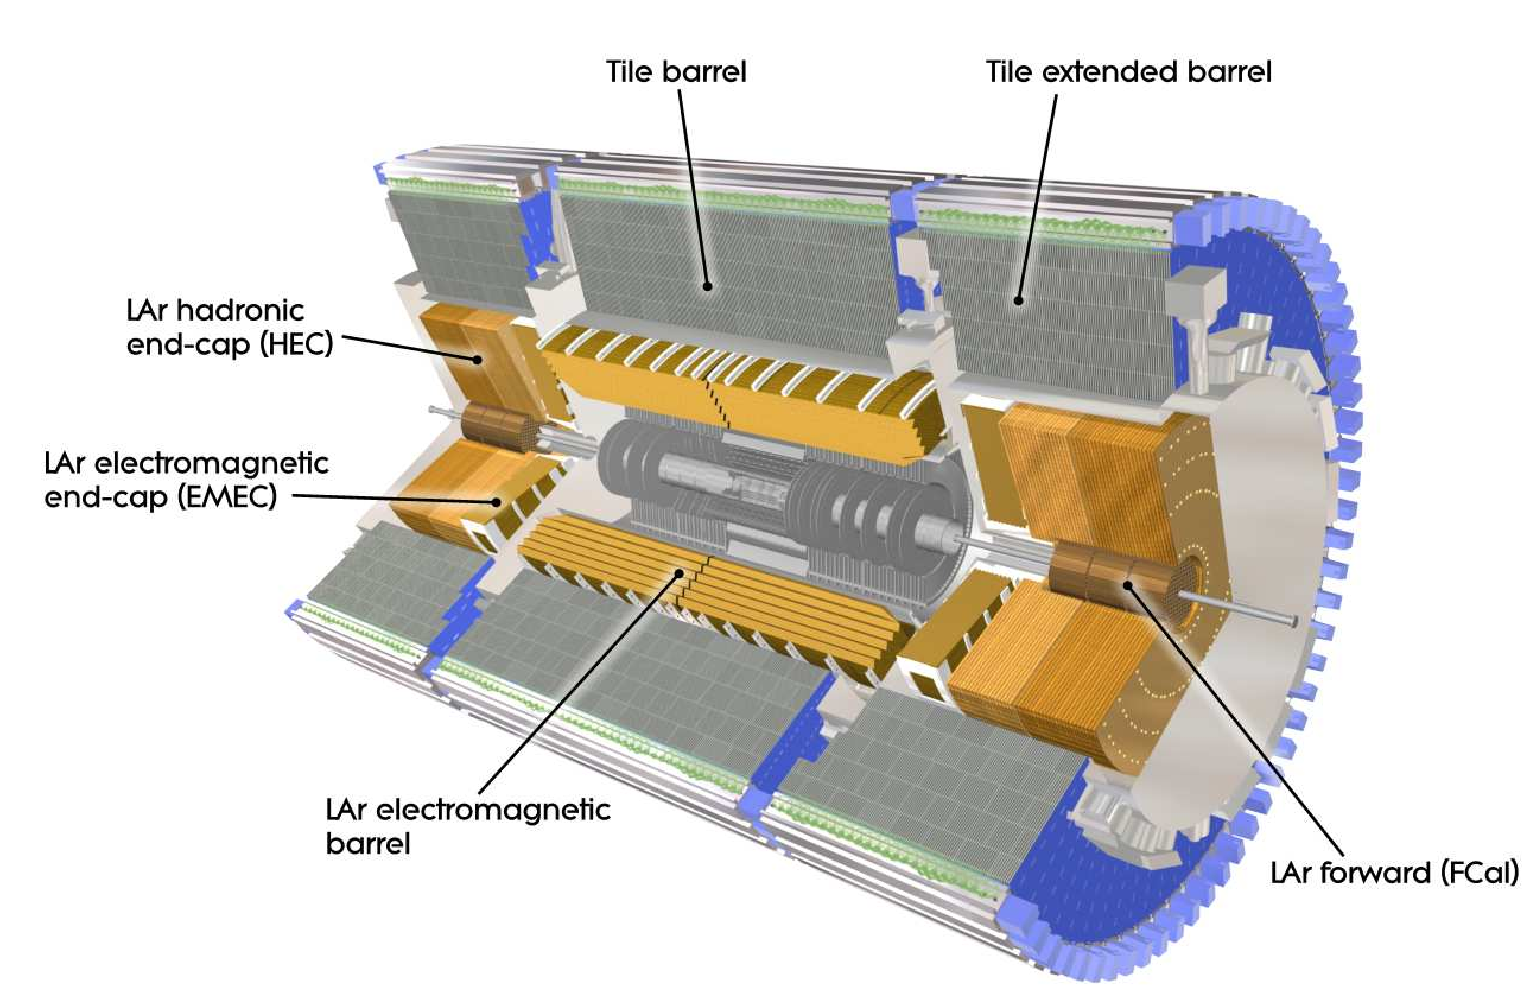
\includegraphics[width=0.8\textwidth]{figure/Calo.png}

    \end{center}
    \caption{Cut-away view of the ATLAS calorimeter system~\cite{ATLASDetector}.}



   \label{fig:atlasCal}
\end{figure}

An illustration of the ATLAS calorimeter system is given in Figure~\ref{fig:atlasCal}. It consists of an electromagnetic calorimeter (EM) 
surrounded by a hadron calorimeter which cover the pseudorapidity 
range $|\eta| < 4.9$.
%
%using different techniques suited to the
%widely varying  radiation environment over this large $\eta-$range. 
Both  calorimeters are sampling calorimeters alternating passive absorber plates to active material 
where the signals are produced.
The total detector material  at $\eta = 0$ corresponds to 9.7 hadronic interaction length $\lambda$. 

The liquid-argon (LAr) EM calorimeter is ideally suited for precision measurement of electron and photon
energies. Liquid argon is used as  active material while lead is used as absorber. The EM calorimeter extends up to $|\eta| = 3.2\,.$
The total thickness of the EM calorimeter is about 22 radiation lengths in the barrel and greater than 24 in the
end-caps. In the barrel part, it is divided in depth into three cylindrical layers 
which are  segmented into $\eta-\phi$ cells of varying  size depending on the layer and 
on pseudorapidity. The $\phi$ cell sizes  rage from  0.025 to 0.1, while the $\eta$ sizes range 
from 0.0035 to 0.075\,.
The energy resolutions for electrons and for 
photons are ranges from $9-22$\%/$\sqrt{E}$ and from $8-14$\%/$\sqrt{E}$, respectively, depending on
pseudorapidity.

The hadron calorimeter has a coarser granularity than the EM calorimeter and  serves  for the 
reconstruction of hadron jets and the measurement of the missing transverse energy. It 
is divided into three sub-detector systems which  use different technologies to cope 
with the $\eta$-dependent radiation environment. The tile calorimeter covers the pseudorapidity range  $|\eta| < 1.7\,$. 
Scintillating tiles are employed as active material and steel as absorber. 
In the end-cap regions,  a LAr hadron  calorimeter (HEC) is used 
which extends up to $|\eta| = 3.2$ and uses Argon as  active and copper as absorber material. 
The  forward regions at  $3.1 <|\eta| < 4.9$ are instrumented  with 
liquid-Argon Forward CALorimeters (FCAL)  
%this provides clear benefits in terms of uniformity of the calorimetric coverage as well as
%reduced radiation background levels in the muon spectrometer. 
which are divided into three modules. In the module closest to the interaction point, copper is used as absorber material, 
while the other two modules employ tungsten.
The jet energy resolution in the barrel is  about 15\% for jets with $\pt=50$~GeV and 
 about 7\% for jets with $\pt=1$~TeV~\cite{jer}.


\subsection{The Muon Spectrometer}
\begin{figure}[tp]
     \begin{center}

            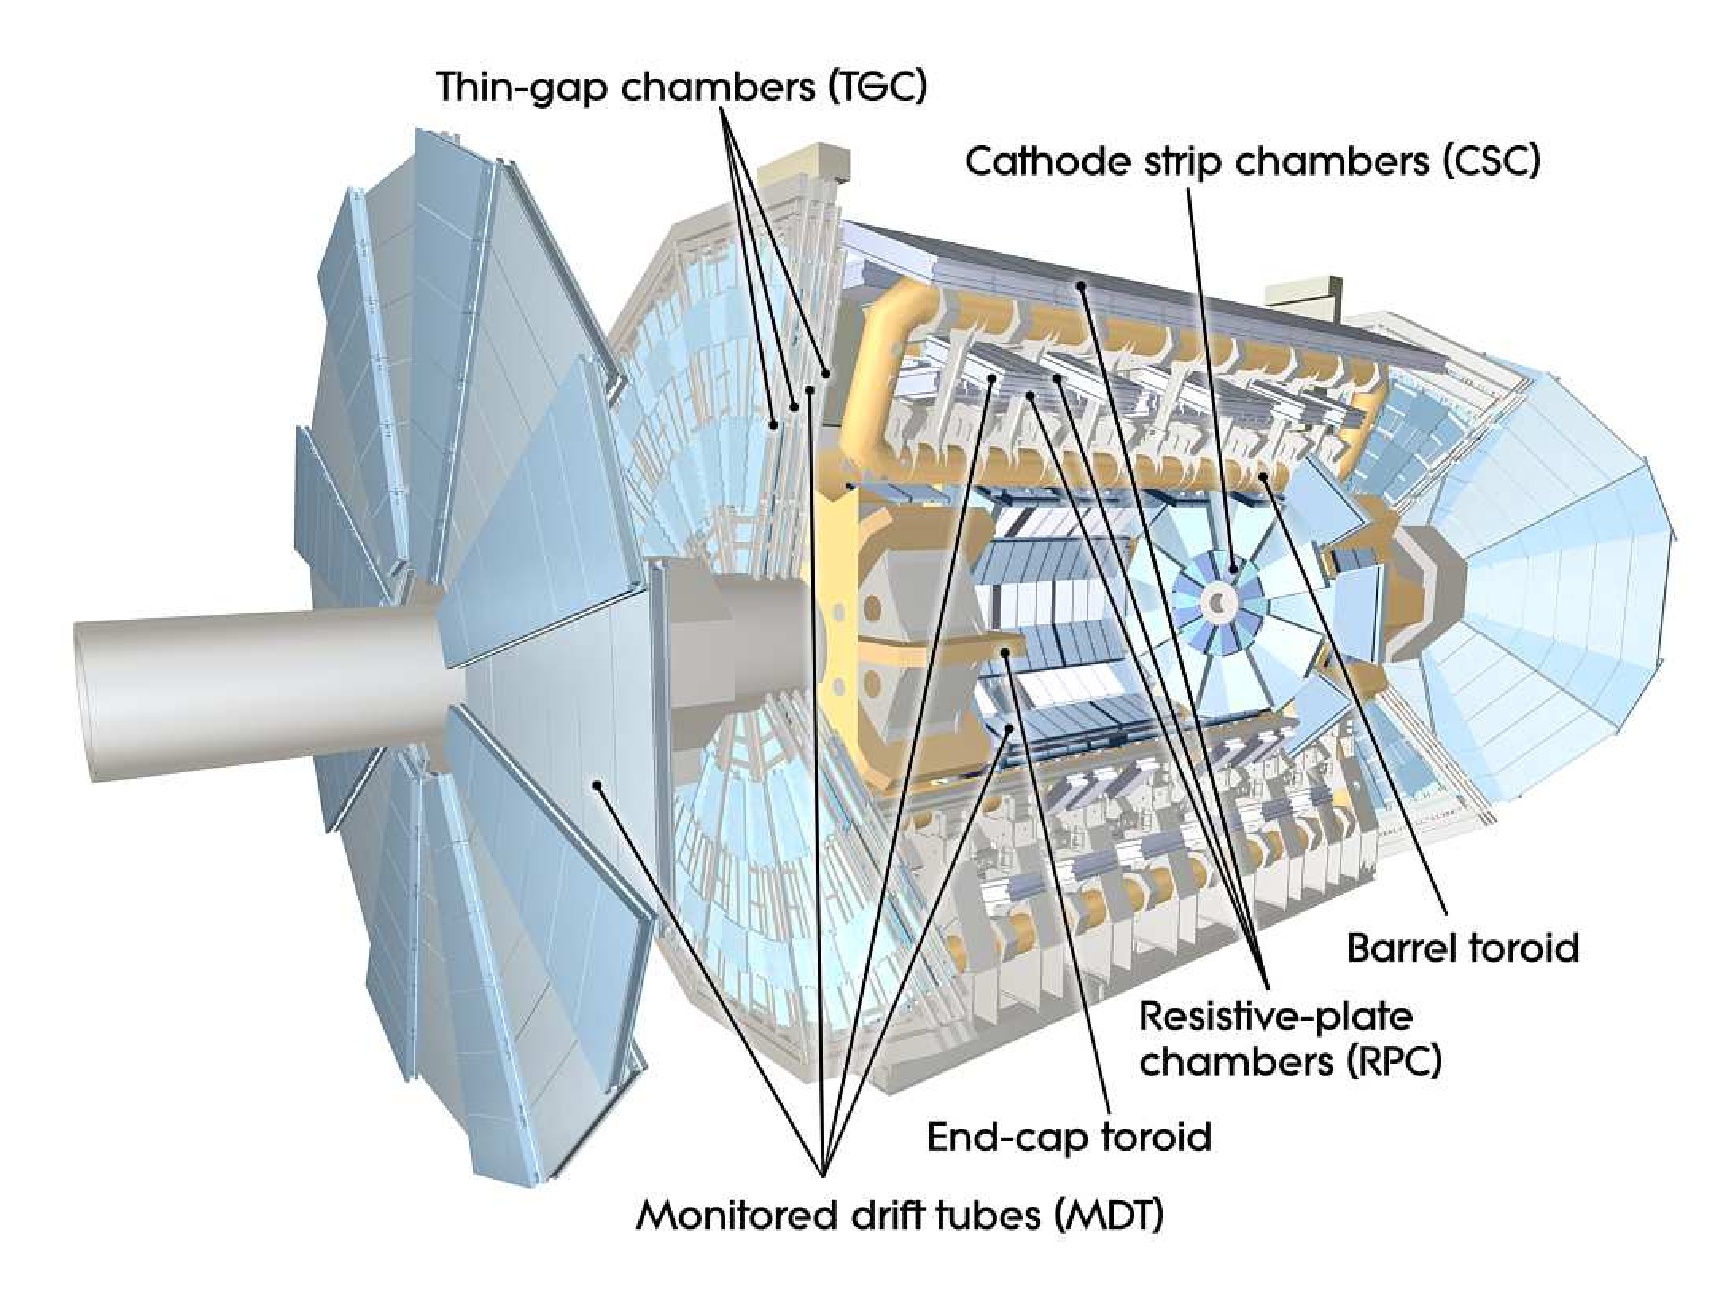
\includegraphics[width=0.8\textwidth]{figure/muonSpec.png}

    \end{center}
    \caption{Cut-away view of the ATLAS muon spectrometer system~\cite{ATLASDetector}.}



   \label{fig:atlasMu}
\end{figure}
The muon spectrometer is instrumented with separate high-precision tracking and muon trigger chambers. 
The muon momenta are measured  by reconstructing the  curvature of the muon trajectory in a
 toroidal magnetic field of 0.3-1.2\,T  which is  produced by large superconducting air-core toroid magnets.
The layout of the muon spectrometer is shown in Figure~\ref{fig:atlasMu}.

Precision measurement of the track coordinates in the bending plane of the 
magnetic field is provided by three layers of Monitored Drift Tube (MDT) chambers covering the pseudo rapidity range
 $|\eta| < 2.7\,.$ Because of the high background rates at large pseudo rapidities, 
$|\eta| > 2$, Cathode Strip Chambers (CSC) are used close to the beam-pipe in the inner end-cap layers. 
The CSC are multi-wire proportional chambers with cathodes segmented into strips. 
The muon spectrometer allows for a muon momentum resolution of better than 10\%  for momenta up to 1~TeV.
The best momentum resolution of 3-4\% is achieved for muons with transverse momenta of about $100$~GeV. 

The muon trigger chambers cover the pseudo rapidity range $|\eta| < 2.4\,.$ Resistive Plate Chambers
(RPC) are used  in the barrel and Thin Gap Chambers (TGC) in the end-cap regions
provide a relatively coarse but fast muon momentum measurement for the Level-1 muon trigger.


\subsection{The Trigger System}
At a nominal LHC  bunch crossing rate of 40~MHz, it is impossible to record and store 
the data of each bunch crossing. A highly selective  trigger system is designed to reduce the initial rate to about 300~Hz
keeping the interesting events. The triggering is performed in three stages with increasing sophistication: the
Level-1 (L1), the Level~2 (L2) triggers and the event filter (EF). Each trigger level
refines the decisions made at the previous level.

The L1 trigger is hardware based and  designed to reach a decision within a latency of less than 2.5 $\mu$s reducing the initial
rate to about 75~KHz. It  relies on coarse energy measurement in the calorimeters and on muon 
momenta information provided by the RPC and TGC chambers. It selects
high transverse-momentum muons, electrons, photons, jets and  $\tau$ 
leptons decaying into hadrons, as well as large missing and total transverse energy.
The L1 defines in each triggered event regions of interest (RoI) 
in  $\eta$ and $\phi$ which are further investigated by the higher-level triggers.

The L2 trigger  selection is seeded by the RoI information provided by the L1 trigger. Unlike the L1 trigger,
the L2 trigger uses the full detector granularity within the RoIs allowing for a more precise reconstruction of particle properties.
The L2 triggers  reduce the event rate to approximately $3.5\,\text{kHz}$.

The final stage of the event selection is the event filter which reduces
the event rate to 300~Hz. It uses the offline reconstruction algorithms described in Chapter~\ref{chap:obj}$\,$.


\subsection{Luminosity Measurement}
A precise measurement of the recorded instantaneous and integrated luminosity is essential for
all  physics studies.
Several luminosity measurement techniques are employed as described in ~\cite{luminosity}.
The detectors relevant for the luminosity monitoring are the inner detector,
the beam conditions monitor (BCM)~\cite{luminosity} and the LUCID detector~\cite{lucid}. 
The inner detector provides a 
luminosity measurement from  the average number of reconstructed proton-proton interactions per bunch crossing.
The LUCID detector surrounds the beam pipe on both sides of the interaction point at a distance of 17 m. It consist of
Cherenkov detectors which  measure  the particle flux from the interaction point in  very forward 
direction. The BCM detector consists of four small diamond sensors  arranged around the beam pipe in a cross pattern
on each side of the interaction point.
It is a fast detector primarily designed to monitor the beam condition which also provides an independent luminosity 
determination. The overall uncertainty in the luminosity measurement using 
these methods is about 3\%.























